\documentclass[letterpaper, 12pt]{article}

%%%%%%%%%%%%%%%%%%%%%%%%%%%%%
% DEFINITIONS
\gdef\mytitle{BestShift}
\gdef\mythema{Diplomarbeit}

\gdef\myauthor{BestShift}

\gdef\myversion{1.1}
\gdef\mybegin{\today}
\gdef\myfinish{\today}

%%%%%%%%%%%%%%%%%%%%%%%%%%%%%%
% SETTINGS
\usepackage[in]{fullpage}
\usepackage[T1]{fontenc}
\usepackage[utf8x]{inputenc}
\usepackage[ngerman]{babel}
\usepackage{graphicx} 
\usepackage{textcomp}
\usepackage{sectsty}
\usepackage{caption}
\usepackage{array}
\usepackage{colortbl}
\usepackage{footmisc}
\usepackage{fancyhdr}
\usepackage{ccicons}
\usepackage{suffix}
\usepackage{multirow}
\usepackage{tabularx}
\usepackage{color}
\usepackage{url}
\usepackage{setspace}
\usepackage{enumitem}
\usepackage{listings}
\usepackage{xcolor}
\usepackage{filecontents}
\usepackage{glossaries}
\usepackage{titlesec}
\usepackage{mhchem}
\usepackage{wrapfig}
\usepackage{accsupp}
\usepackage[export]{adjustbox}
\usepackage{dirtree}
\usepackage[headsep=1cm,headheight=3cm,hmargin=2cm,vmargin=2.5cm]{geometry}
\usepackage[nolist]{acronym}
\usepackage[toc,page]{appendix}

\usepackage[
	colorlinks,
	citecolor=black,
	filecolor=black,
	linkcolor=black,
	urlcolor=black,
	linktoc=all
]{hyperref}

%%%%%%%%%%%%%%%%%%%%%%%%%%%%%%%%%%%%%%%%%%%%%%%%%%%%%%%%%%%%%%%
%% Useful commands

% Comments and notes

\newtoggle{devel}
%\toggletrue{devel}
\togglefalse{devel}

\iftoggle{devel} {
	\newcommand{\comment}[1]{{\bf \colorbox{yellow}{\color{black}#1}}\nextline}
	\newcommand{\todo}[1]{{\bf \colorbox{red}{\color{white}TODO: #1}}\nextline}	
} {
	\newcommand{\comment}[1]{{}}
	\newcommand{\todo}[1]{{}}
}

\newcommand{\ifreport}[1]{#1}
\newcommand{\ie}{{\em i.e.,~}}
\newcommand{\eg}{{\em e.g.,~}}
\newcommand{\term}[1]{\mbox{\texttt{#1}}}
\newcommand{\itl}[1]{\mbox{\textit{#1}}}

% Commas and semicolons
\newcommand{\comma}{,\,}
\newcommand{\commadots}{\comma \ldots \comma}
\newcommand{\semi}{;\mbox{;};}
\newcommand{\semidots}{\semi \ldots \semi}

% Brackets
\newcommand{\set}[1]{\{#1\}}
\newcommand{\sbs}[1]{\lquote #1 \rquote}

% Spacing
\newcommand{\gap}{\quad\quad}
\newcommand{\biggap}{\quad\quad\quad}
\newcommand{\nextline}{\\ \\}
\newcommand{\htabwidth}{0.5cm}
\newcommand{\tabwidth}{1cm}
\newcommand{\htab}{\hspace{\htabwidth}}
\newcommand{\tab}{\hspace{\tabwidth}}
\newcommand{\linesep}{\ \hrulefill \ \smallskip}

%%%%%%%%%%%%%%%%%%%%%%%%%%%%%%%%%%%%%%%%%%%%%%%%%%%%%%%%%%%%%%%%
%% Settings and tweaks

% use citep instead of cite
%\let\cite\citep
\newcommand{\sectionbreak}{\clearpage}


%Bibtex
\def\BibTeX{{\rm B\kern-.05em{\sc i\kern-.025em b}\kern-.08em
		T\kern-.1667em\lower.7ex\hbox{E}\kern-.125emX}}

%%%%%%%%%%%%%%%%%%%%%%%%%%%%%%%%%%%%%%%%%%%%%%%%%%%%%%%%%%%%%%%%
%% The following listings environments are provided:
%%
%% python     for Python code
%% xml        for XML code
%% bash       for BASH code
%% java       for Java code
%% javascript for javascript code
%%
%% This style file is based on original work by Olivier Verdier,
%% with contributions from Johan Hake.
%%
%% Modified for ANS by Anders Logg, 2011.
%% 
%% The original can be found here
%% http://www.math.chalmers.se/Math/Grundutb/CTH/tmv225/1415/dokument/rapportmall/anslistings.sty 
%%
%% First added:   2015-02-08
%% Last modified: 2015-02-08

% Basic setup
\renewcommand{\lstlistlistingname}{Code Listings}
\renewcommand{\lstlistingname}{Code Listing}
\newcommand{\codetitlestyle}[1]{\small\textit{#1}}
\newcommand{\belowtitleskip}{2pt}
\newcommand{\captionposition}{t}
\newcommand{\framemargin}{0.5ex}
\newcommand{\literatecolour}{\textcolor{literatecolour}}

% Colors
\definecolor{gray}{gray}{0.5}
\definecolor{lightgray}{rgb}{.9,.9,.9}
\definecolor{darkgray}{rgb}{.4,.4,.4}
\definecolor{dkblue}{rgb}{0,0,0.5}
\definecolor{comment}{rgb}{1,0,0}
\definecolor{mauve}{rgb}{.627,.126,.941}
\definecolor{purple}{rgb}{0.5, 0, 0.545098}

\colorlet{commentcolour}{green!50!black}
\colorlet{stringcolour}{red!60!black}
\colorlet{keywordcolour}{magenta!90!black}
\colorlet{exceptioncolour}{yellow!50!red}
\colorlet{commandcolour}{blue!60!black}
\colorlet{numpycolour}{blue!60!green}
\colorlet{literatecolour}{magenta!90!black}
\colorlet{promptcolour}{green!50!black}
\colorlet{specmethodcolour}{violet}
\colorlet{indendifiercolour}{green!70!white}


\lstdefinelanguage{JavaScript}{
  keywords={break, case, catch, continue, debugger, default, delete, do, else, false, finally, for, function, if, in, instanceof, new, null, return, switch, this, throw, true, try, typeof, var, void, while, with},
  morecomment=[l]{//},
  morecomment=[s]{/*}{*/},
  morestring=[b]',
  morestring=[b]",
  ndkeywords={class, export, boolean, throw, implements, import, this},
  keywordstyle=\color{blue}\bfseries,
  ndkeywordstyle=\color{darkgray}\bfseries,
  identifierstyle=\color{black},
  commentstyle=\color{purple}\ttfamily,
  stringstyle=\color{red}\ttfamily,
  sensitive=true
}

\lstset{
   language=JavaScript,
   backgroundcolor=\color{lightgray},
   extendedchars=true,
   basicstyle=\footnotesize\ttfamily,
   showstringspaces=false,
   showspaces=false,
   numbers=none,
   tabsize=2,
   breaklines=true,
   showtabs=false,
   captionpos=b
}

%--- Typesetting Java ---

\lstdefinestyle{javastyle}{
  belowcaptionskip=1\baselineskip,
  breakatwhitespace=false,        % sets if automatic breaks should only happen at whitespace
  breaklines=true,                % sets automatic line breaking
  xleftmargin=1cm,
  language=Java,
  tabsize=4, 
  tabsize=4,
  numbers=left,
  showstringspaces=false,
  keywordstyle=\color{keywordcolour}\bfseries,
  commentstyle=\color{commentcolour}\slshape,
  numberstyle=\tiny\noncopynumber,
  basicstyle=\footnotesize\ttfamily,
  keywordstyle=\bfseries\color[rgb]{.133,.545,.133},
  commentstyle=\itshape\color{blue},
  stringstyle=\color{mauve},
  %directivestyle=\bfseries\color{purple},
  frame=single],
  resetmargins=true,
}

\newcommand{\noncopynumber}[1]{%
\BeginAccSupp{method=escape,ActualText={}}%
#1%
\EndAccSupp{}%
}

\newcommand{\inputjava}[1]{\lstinputlisting[style=javastyle,title={\codetitlestyle{Java code }},belowcaptionskip=\belowtitleskip]{#1}}
\lstnewenvironment{java}[1][]{\lstset{style=javastyle,title={\codetitlestyle{Java code }},belowcaptionskip=\belowtitleskip}}{}
\newcommand{\javac}{\lstinline[style=javastyle,basicstyle=\ttfamily]}

%--- Typesetting Python ---

 \lstdefinestyle{pythonstyle}{
 language=python,
 showtabs=true,
 tab=,
 tabsize=2,
 basicstyle=\ttfamily\footnotesize,
 stringstyle=\color{stringcolour},
 showstringspaces=false,
 alsoletter={1234567890},
 otherkeywords={\ , \}, \{, \%, \&, \|},
 keywordstyle=\color{keywordcolour}\bfseries,
 emph={and,break,class,continue,def,yield,del,elif ,else,%
 except,exec,finally,for,from,global,if,import,in,%
 lambda,not,or,pass,print,raise,return,try,while,assert},
 emphstyle=\color{blue}\bfseries,
 emph={[2]True, False, None},
 emphstyle=[2]\color{keywordcolour},
 emph={[3]object,type,isinstance,copy,deepcopy,zip,enumerate,reversed,list,len,dict,tuple,xrange,append,execfile,real,imag,reduce,str,repr},
 emphstyle=[3]\color{commandcolour},
 emph={Exception,NameError,IndexError,SyntaxError,TypeError,ValueError,OverflowError,ZeroDivisionError},
 emphstyle=\color{exceptioncolour}\bfseries,
 commentstyle=\color{commentcolour}\slshape,
 emph={[4]ode, fsolve, sqrt, exp, sin, cos, arccos, pi,  array, norm, solve, dot, arange, , isscalar, max, sum, flatten, shape, reshape, find, any, all, abs, plot, linspace, legend, quad, polyval,polyfit, hstack, concatenate,vstack,column_stack,empty,zeros,ones,rand,vander,grid,pcolor,eig,eigs,eigvals,svd,qr,tan,det,logspace,roll,min,mean,cumsum,cumprod,diff,vectorize,lstsq,cla,eye,xlabel,ylabel,squeeze},
 emphstyle=[4]\color{numpycolour},
 emph={[5]__init__,__add__,__mul__,__div__,__sub__,__call__,__getitem__,__setitem__,__eq__,__ne__,__nonzero__,__rmul__,__radd__,__repr__,__str__,__get__,__truediv__,__pow__,__name__,__future__,__all__},
 emphstyle=[5]\color{specmethodcolour},
 emph={[6]assert,range,yield},
 emphstyle=[6]\color{keywordcolour}\bfseries,
 literate=*%
 {:}{{\literatecolour:}}{1}%
 {=}{{\literatecolour=}}{1}%
 {-}{{\literatecolour-}}{1}%
 {+}{{\literatecolour+}}{1}%
 {*}{{\literatecolour*}}{1}%
 {/}{{\literatecolour/}}{1}%
 {!}{{\literatecolour!}}{1}%
 {[}{{\literatecolour[}}{1}%
 {]}{{\literatecolour]}}{1}%
 {<}{{\literatecolour<}}{1}%
 {>}{{\literatecolour>}}{1}%
 {>>>}{{\textcolor{promptcolour}{>>>}}}{1}%
 ,%
 breaklines=true,
 breakatwhitespace= true,
 aboveskip=1ex,
 frame=trbl,
 framesep=.3ex,
 rulecolor=\color{black!40}
}

\newcommand{\inputpython}[1]{\lstinputlisting[style=pythonstyle,title={\codetitlestyle{Python code }},belowcaptionskip=\belowtitleskip]{#1}}
\lstnewenvironment{python}[1][]{\lstset{style=pythonstyle,title={\codetitlestyle{Python code }},belowcaptionskip=\belowtitleskip}}{}
\newcommand{\pyth}{\lstinline[style=pythonstyle,basicstyle=\ttfamily]}

%--- Typesetting XML ---

\lstdefinestyle{xmlstyle}{
language=xml,
showtabs=true,
tab=,
tabsize=2,
basicstyle=\ttfamily\footnotesize,
stringstyle=\color{stringcolour},
showstringspaces=false,
alsoletter={1234567890},
emphstyle=\color{exceptioncolour}\bfseries,
commentstyle=\color{commentcolour}\slshape,
breaklines=true,
breakatwhitespace= true,
aboveskip=1ex,
frame=trbl,
framesep=.3ex,
rulecolor=\color{black!40}
}

\newcommand{\inputxml}[1]{\lstinputlisting[style=xmlstyle, title={\codetitlestyle{XML code}}, belowcaptionskip=\belowtitleskip]{#1}}
\lstnewenvironment{xml}[1][]{\lstset{style=xmlstyle, title={\codetitlestyle{XML code}}, belowcaptionskip=\belowtitleskip}}{}

%--- Typesetting Bash ---

\lstdefinestyle{bashstyle}{
language=bash,
showtabs=true,
tab=,
tabsize=2,
basicstyle=\ttfamily\footnotesize,
stringstyle=\color{stringcolour},
showstringspaces=false,
alsoletter={1234567890},
otherkeywords={\ , \}, \{, \%, \&, \|},
emphstyle=\color{exceptioncolour}\bfseries,
commentstyle=\color{commentcolour}\slshape,
breaklines=true,
breakatwhitespace= true,
aboveskip=1ex,
frame=trbl,
framesep=.3ex,
rulecolor=\color{black!40}
}

\newcommand{\inputbash}[1]{\lstinputlisting[style=bashstyle, title={\codetitlestyle{Bash code}}, belowcaptionskip=\belowtitleskip]{#1}}
\lstnewenvironment{bash}[1][]{\lstset{style=bashstyle, title={\codetitlestyle{Bash code}}, belowcaptionskip=\belowtitleskip}}{}
\lstnewenvironment{csh}[1][]{\lstset{style=bashstyle, title={\codetitlestyle{Csh code}}, belowcaptionskip=\belowtitleskip}}{}

\linespread{0.94}
\lhead{Diplomarbeit}
\chead{}
\rhead{Version \myversion}
\cfoot{\thepage}
\rfoot{\ccby\hspace{2mm}\myauthor}
\renewcommand{\headrulewidth}{0.4pt}
\renewcommand{\footrulewidth}{0.4pt}

%%%%%%%%%%%%%%%%%%%%%%%%%%%%%
% DOCUMENT BEGIN
\begin{document}
\parindent 0pt
\parskip 6pt

% TITLE PAGE
\begin{titlepage}

	\begin{figure}[h]
		\makebox[\textwidth]{%
		
\includegraphics[width=0.25\linewidth]{images/bestshift_logo.png}%
		\hfill    
		
\includegraphics[width=0.3\linewidth]{images/jdIT_tgm.png}%
		}\\[0.5cm]% If you want some vertical space
	\end{figure}

	\vspace{1.5cm} 

	{\begin{center} \bfseries\huge
			\rule{17.5cm}{0.1mm}  
			\\[5mm]
			\mytitle\\[5mm]
			\mythema\\
			\rule{17.5cm}{0.1mm}  
	\end{center}}

	\vspace{0.1cm} 

	{\begin{table}[!h] \bfseries\normalsize
		\begin{tabularx}{\textwidth}{lXr @{\hspace{0mm}}}
			Hüseyin Bozkurt - Fitim Faiku - Daniel Melichar - Tobias Perny - Raphael Simsek\\[10mm]
		\end{tabularx}
	\end{table}}

	\vspace{2cm} 

	{\begin{table}[!h] \bfseries\normalsize
		\begin{tabularx}{\textwidth}{lXr @{\hspace{0mm}}}
			&& Version \myversion\\
			&& \mybegin\\
		\end{tabularx}
	\end{table}}


	{\begin{table}[!h] \bfseries\normalsize
		\begin{tabularx}{\textwidth}{lXr @{\hspace{0mm}}}
			&& Technologisches Gewerbemuseum\\
			&& Abteilung der Informationstechnologie\\
			&& Wien, 2015/16\\[10mm]
		\end{tabularx}
	\end{table}}

\end{titlepage}


% TOC, TABLES, FIGURES, ABSTRACT
\pagenumbering{Roman} 
\clearpage
\tableofcontents
\clearpage
\section*{Abstract}

Lorem ipsum dolor sit amet, consectetur adipisicing elit, sed do eiusmod
tempor incididunt ut labore et dolore magna aliqua. Ut enim ad minim veniam,
quis nostrud exercitation ullamco laboris nisi ut aliquip ex ea commodo
consequat. Duis aute irure dolor in reprehenderit in voluptate velit esse
cillum dolore eu fugiat nulla pariatur. Excepteur sint occaecat cupidatat non
proident, sunt in culpa qui officia deserunt mollit anim id est laborum.
\section*{Anerkennungen}

Wir widmen diese Arbeit jenen Personen die uns gezeigt haben, dass unser Aufwand wertgeschätzt wird; die uns in den schwierigen Phasen unterstützt und motiviert haben; und die uns auch auf einer persönlichen Ebene weitergebracht haben. Insbesondere bedanken wir uns bei Prof. Dipl.-Ing. Heinz Neuburger und unserem unersetzlichen Projektbetreuer Erhard List.
\section*{Eidestattliche Erklärung}
Ich erkläre an Eides statt, dass ich die vorliegende Diplomarbeit selbstständig und ohne fremde Hilfe verfasst, andere als angegebene Quellen und Hilfsmittel nicht benutzt und die benutzten Quellen wörtlich und inhaltlich entommenen Stellen als solche erkenntlich gemacht habe.

\vspace{0.5cm}

Wien, \today

\vspace{1.5cm}

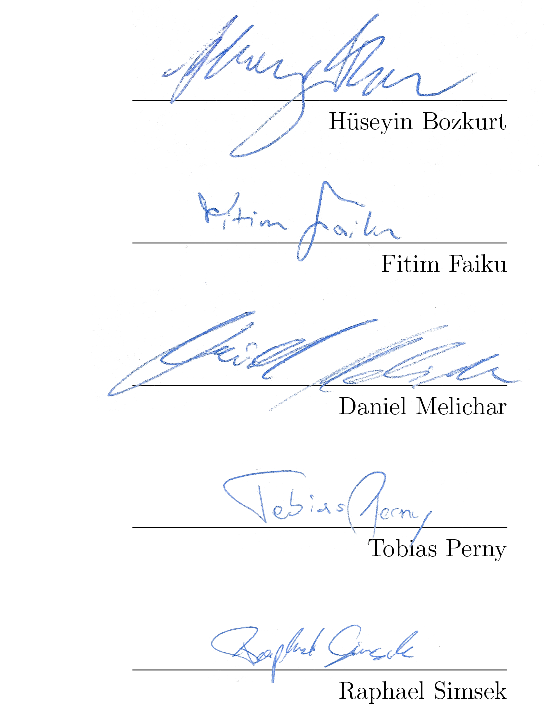
\includegraphics[width=0.5\textwidth, right]{special/eides}

 
% CONTNET
\clearpage
\pagenumbering{arabic}
\pagestyle{fancy}
\section{Technische Grundlagen}
\label{sec:intro}
\lfoot{Autor: Raphael Simsek}

\subsection{CAN - Bus}
\subsubsection{OBD II}
Die OBD-II Schnittstelle ist eine normierte, standardisierte Schnittstelle, welche, mittels einem passenden Auslesegerät, Zugriff auf die Daten den Motormanagements verschafft. Diese Schnittstelle hat unterschiedliche Versionen, welche auf die verschiedenen Kontinente aufgeschlüsselt wurden. Es gibt also OBD II, was Initial eine Schnittstelle der vereinigten Staaten war, weshalb der Standard auch in Nordamerika seit 1996 verbaut wurde. Zusätzlich gibt es EOBD, womit die europäische Umsetzung des OBD II Standards beschrieben wird.\cite{Directive.98/69/EC.EUParliament} Der wesentliche Unterschied ist dabei die Standardisierung, welche zwar technisch zwischen SAE J1962 und ISO/DIS 15031 gleich ist, aber trotzdem unterschiedlich benannt wurde. \cite{SAE.J1962} Ferner gab es eine australische \cite{AU.Motor.Vehicle.Standards.Act.1989} und eine japanische Version der Standardisierung.
\newline
\newline
Ausserdem gibt es eine, ebenfalls in der Standardisierung festgehalten einen OBD II A und B Konnektor. Der A Konnektor ist für alle Fahrzeuge mit 12 V Bordspannung und hat die Form eines D mit einer Nut in der Mitte, um die Pins zu behausen. Der B Konnektor verwendet ebenfalls die Form eines D's, allerdings ist dieser Konnektor für Fahrzeuge mit 24V Bordspannung, was häufig Lastkraftfahrzeuge sind. Bei diesem Konnektor ist die Nut in der Mitte unterbrochen, um es unmöglich zu machen einen männlichen Konnektor des A-Typs einzustecken. Dieser Konnektor könnte folglich nämlich aufgrund von Überspannung defekt werden. Es ist also der B Konnektor sowohl mit A und B kompatibel, allerdings ist der A Konnektor nur mit seinesgleichen verwendbar.


\begin{figure}[!htb]\centering
   \begin{minipage}{0.49\textwidth}
     \frame{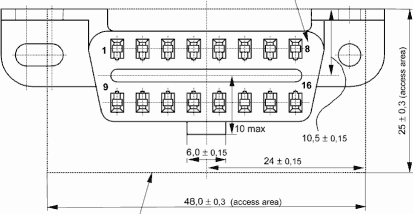
\includegraphics[width=\linewidth]{images/j1962f_type_a}}
     \caption{Typ A, OBD II Konnektor \cite{OBDII.TypeA}}\label{Fig:Data1}
   \end{minipage}
   \begin {minipage}{0.49\textwidth}
     \frame{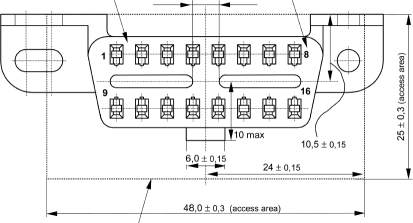
\includegraphics[width=\linewidth]{images/j1962f_type_b}}
     \caption{Typ B, OBD II Konnektor \cite{OBDII.TypeB}}\label{Fig:Data2}
   \end{minipage}
\end{figure}


\section{Technische Grundlagen}
\label{sec:intro}
\lfoot{Autor: Raphael Simsek}

\subsection{CAN - Bus}
\subsubsection{OBD II}
Die OBD-II Schnittstelle ist eine normierte, standardisierte Schnittstelle, welche, mittels einem passenden Auslesegerät, Zugriff auf die Daten den Motormanagements verschafft. Diese Schnittstelle hat unterschiedliche Versionen, welche auf die verschiedenen Kontinente aufgeschlüsselt wurden. Es gibt also OBD II, was Initial eine Schnittstelle der vereinigten Staaten war, weshalb der Standard auch in Nordamerika seit 1996 verbaut wurde. Zusätzlich gibt es EOBD, womit die europäische Umsetzung des OBD II Standards beschrieben wird.\cite{Directive.98/69/EC.EUParliament} Der wesentliche Unterschied ist dabei die Standardisierung, welche zwar technisch zwischen SAE J1962 und ISO/DIS 15031 gleich ist, aber trotzdem unterschiedlich benannt wurde. \cite{SAE.J1962} Ferner gab es eine australische \cite{AU.Motor.Vehicle.Standards.Act.1989} und eine japanische Version der Standardisierung.
\newline
\newline
Ausserdem gibt es eine, ebenfalls in der Standardisierung festgehalten einen OBD II A und B Konnektor. Der A Konnektor ist für alle Fahrzeuge mit 12 V Bordspannung und hat die Form eines D mit einer Nut in der Mitte, um die Pins zu behausen. Der B Konnektor verwendet ebenfalls die Form eines D's, allerdings ist dieser Konnektor für Fahrzeuge mit 24V Bordspannung, was häufig Lastkraftfahrzeuge sind. Bei diesem Konnektor ist die Nut in der Mitte unterbrochen, um es unmöglich zu machen einen männlichen Konnektor des A-Typs einzustecken. Dieser Konnektor könnte folglich nämlich aufgrund von Überspannung defekt werden. Es ist also der B Konnektor sowohl mit A und B kompatibel, allerdings ist der A Konnektor nur mit seinesgleichen verwendbar.


\begin{figure}[!htb]\centering
   \begin{minipage}{0.49\textwidth}
     \frame{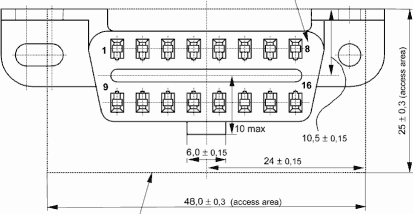
\includegraphics[width=\linewidth]{images/j1962f_type_a}}
     \caption{Typ A, OBD II Konnektor \cite{OBDII.TypeA}}\label{Fig:Data1}
   \end{minipage}
   \begin {minipage}{0.49\textwidth}
     \frame{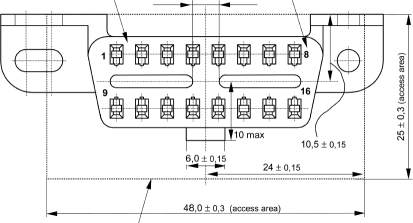
\includegraphics[width=\linewidth]{images/j1962f_type_b}}
     \caption{Typ B, OBD II Konnektor \cite{OBDII.TypeB}}\label{Fig:Data2}
   \end{minipage}
\end{figure}


\section{Technische Grundlagen}
\label{sec:intro}
\lfoot{Autor: Raphael Simsek}

\subsection{CAN - Bus}
\subsubsection{OBD II}
Die OBD-II Schnittstelle ist eine normierte, standardisierte Schnittstelle, welche, mittels einem passenden Auslesegerät, Zugriff auf die Daten den Motormanagements verschafft. Diese Schnittstelle hat unterschiedliche Versionen, welche auf die verschiedenen Kontinente aufgeschlüsselt wurden. Es gibt also OBD II, was Initial eine Schnittstelle der vereinigten Staaten war, weshalb der Standard auch in Nordamerika seit 1996 verbaut wurde. Zusätzlich gibt es EOBD, womit die europäische Umsetzung des OBD II Standards beschrieben wird.\cite{Directive.98/69/EC.EUParliament} Der wesentliche Unterschied ist dabei die Standardisierung, welche zwar technisch zwischen SAE J1962 und ISO/DIS 15031 gleich ist, aber trotzdem unterschiedlich benannt wurde. \cite{SAE.J1962} Ferner gab es eine australische \cite{AU.Motor.Vehicle.Standards.Act.1989} und eine japanische Version der Standardisierung.
\newline
\newline
Ausserdem gibt es eine, ebenfalls in der Standardisierung festgehalten einen OBD II A und B Konnektor. Der A Konnektor ist für alle Fahrzeuge mit 12 V Bordspannung und hat die Form eines D mit einer Nut in der Mitte, um die Pins zu behausen. Der B Konnektor verwendet ebenfalls die Form eines D's, allerdings ist dieser Konnektor für Fahrzeuge mit 24V Bordspannung, was häufig Lastkraftfahrzeuge sind. Bei diesem Konnektor ist die Nut in der Mitte unterbrochen, um es unmöglich zu machen einen männlichen Konnektor des A-Typs einzustecken. Dieser Konnektor könnte folglich nämlich aufgrund von Überspannung defekt werden. Es ist also der B Konnektor sowohl mit A und B kompatibel, allerdings ist der A Konnektor nur mit seinesgleichen verwendbar.


\begin{figure}[!htb]\centering
   \begin{minipage}{0.49\textwidth}
     \frame{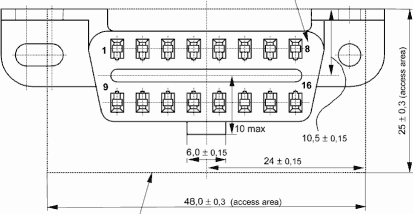
\includegraphics[width=\linewidth]{images/j1962f_type_a}}
     \caption{Typ A, OBD II Konnektor \cite{OBDII.TypeA}}\label{Fig:Data1}
   \end{minipage}
   \begin {minipage}{0.49\textwidth}
     \frame{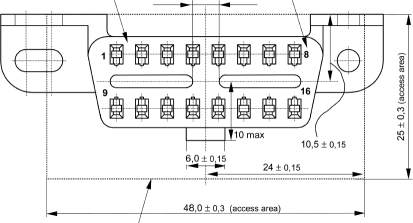
\includegraphics[width=\linewidth]{images/j1962f_type_b}}
     \caption{Typ B, OBD II Konnektor \cite{OBDII.TypeB}}\label{Fig:Data2}
   \end{minipage}
\end{figure}


\section{Technische Grundlagen}
\label{sec:intro}
\lfoot{Autor: Raphael Simsek}

\subsection{CAN - Bus}
\subsubsection{OBD II}
Die OBD-II Schnittstelle ist eine normierte, standardisierte Schnittstelle, welche, mittels einem passenden Auslesegerät, Zugriff auf die Daten den Motormanagements verschafft. Diese Schnittstelle hat unterschiedliche Versionen, welche auf die verschiedenen Kontinente aufgeschlüsselt wurden. Es gibt also OBD II, was Initial eine Schnittstelle der vereinigten Staaten war, weshalb der Standard auch in Nordamerika seit 1996 verbaut wurde. Zusätzlich gibt es EOBD, womit die europäische Umsetzung des OBD II Standards beschrieben wird.\cite{Directive.98/69/EC.EUParliament} Der wesentliche Unterschied ist dabei die Standardisierung, welche zwar technisch zwischen SAE J1962 und ISO/DIS 15031 gleich ist, aber trotzdem unterschiedlich benannt wurde. \cite{SAE.J1962} Ferner gab es eine australische \cite{AU.Motor.Vehicle.Standards.Act.1989} und eine japanische Version der Standardisierung.
\newline
\newline
Ausserdem gibt es eine, ebenfalls in der Standardisierung festgehalten einen OBD II A und B Konnektor. Der A Konnektor ist für alle Fahrzeuge mit 12 V Bordspannung und hat die Form eines D mit einer Nut in der Mitte, um die Pins zu behausen. Der B Konnektor verwendet ebenfalls die Form eines D's, allerdings ist dieser Konnektor für Fahrzeuge mit 24V Bordspannung, was häufig Lastkraftfahrzeuge sind. Bei diesem Konnektor ist die Nut in der Mitte unterbrochen, um es unmöglich zu machen einen männlichen Konnektor des A-Typs einzustecken. Dieser Konnektor könnte folglich nämlich aufgrund von Überspannung defekt werden. Es ist also der B Konnektor sowohl mit A und B kompatibel, allerdings ist der A Konnektor nur mit seinesgleichen verwendbar.


\begin{figure}[!htb]\centering
   \begin{minipage}{0.49\textwidth}
     \frame{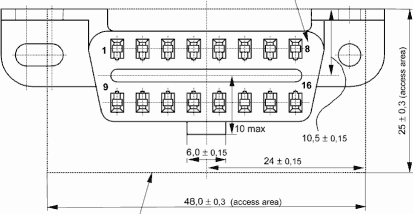
\includegraphics[width=\linewidth]{images/j1962f_type_a}}
     \caption{Typ A, OBD II Konnektor \cite{OBDII.TypeA}}\label{Fig:Data1}
   \end{minipage}
   \begin {minipage}{0.49\textwidth}
     \frame{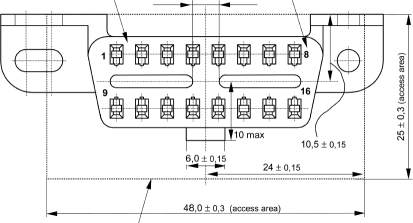
\includegraphics[width=\linewidth]{images/j1962f_type_b}}
     \caption{Typ B, OBD II Konnektor \cite{OBDII.TypeB}}\label{Fig:Data2}
   \end{minipage}
\end{figure}


\section{Technische Grundlagen}
\label{sec:intro}
\lfoot{Autor: Raphael Simsek}

\subsection{CAN - Bus}
\subsubsection{OBD II}
Die OBD-II Schnittstelle ist eine normierte, standardisierte Schnittstelle, welche, mittels einem passenden Auslesegerät, Zugriff auf die Daten den Motormanagements verschafft. Diese Schnittstelle hat unterschiedliche Versionen, welche auf die verschiedenen Kontinente aufgeschlüsselt wurden. Es gibt also OBD II, was Initial eine Schnittstelle der vereinigten Staaten war, weshalb der Standard auch in Nordamerika seit 1996 verbaut wurde. Zusätzlich gibt es EOBD, womit die europäische Umsetzung des OBD II Standards beschrieben wird.\cite{Directive.98/69/EC.EUParliament} Der wesentliche Unterschied ist dabei die Standardisierung, welche zwar technisch zwischen SAE J1962 und ISO/DIS 15031 gleich ist, aber trotzdem unterschiedlich benannt wurde. \cite{SAE.J1962} Ferner gab es eine australische \cite{AU.Motor.Vehicle.Standards.Act.1989} und eine japanische Version der Standardisierung.
\newline
\newline
Ausserdem gibt es eine, ebenfalls in der Standardisierung festgehalten einen OBD II A und B Konnektor. Der A Konnektor ist für alle Fahrzeuge mit 12 V Bordspannung und hat die Form eines D mit einer Nut in der Mitte, um die Pins zu behausen. Der B Konnektor verwendet ebenfalls die Form eines D's, allerdings ist dieser Konnektor für Fahrzeuge mit 24V Bordspannung, was häufig Lastkraftfahrzeuge sind. Bei diesem Konnektor ist die Nut in der Mitte unterbrochen, um es unmöglich zu machen einen männlichen Konnektor des A-Typs einzustecken. Dieser Konnektor könnte folglich nämlich aufgrund von Überspannung defekt werden. Es ist also der B Konnektor sowohl mit A und B kompatibel, allerdings ist der A Konnektor nur mit seinesgleichen verwendbar.


\begin{figure}[!htb]\centering
   \begin{minipage}{0.49\textwidth}
     \frame{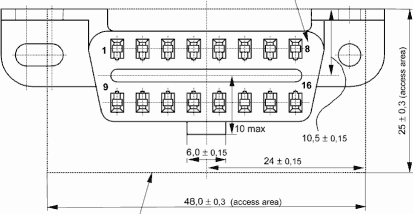
\includegraphics[width=\linewidth]{images/j1962f_type_a}}
     \caption{Typ A, OBD II Konnektor \cite{OBDII.TypeA}}\label{Fig:Data1}
   \end{minipage}
   \begin {minipage}{0.49\textwidth}
     \frame{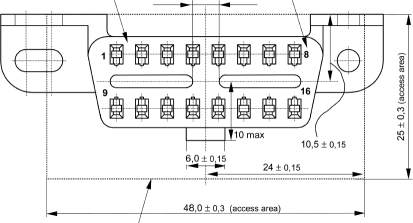
\includegraphics[width=\linewidth]{images/j1962f_type_b}}
     \caption{Typ B, OBD II Konnektor \cite{OBDII.TypeB}}\label{Fig:Data2}
   \end{minipage}
\end{figure}



% Reset Autor
\lfoot{}

% BIBL
\clearpage
\begingroup
\bibliographystyle{abbrv}
\bibliography{sources.bib}
\endgroup

% APPENDENCIES
\clearpage
\pagenumbering{Roman}
\section{Appendix}

\subsection{Figuren}
	\begingroup
		\makeatletter
		\@starttoc{lof}% Print List of Figures
		\makeatother
	\endgroup

\subsection{Tabellen}
	\begingroup
		\makeatletter
		\@starttoc{lot}% Print List of Tables
		\makeatother
	\endgroup

\subsection{Listings}
	\begingroup
		\makeatletter
		\@starttoc{lol}% Print List of Listings lol
		\makeatother
	\endgroup
\end{document}

